\documentclass[1p]{elsarticle_modified}
%\bibliographystyle{elsarticle-num}

%\usepackage[colorlinks]{hyperref}
%\usepackage{abbrmath_seonhwa} %\Abb, \Ascr, \Acal ,\Abf, \Afrak
\usepackage{amsfonts}
\usepackage{amssymb}
\usepackage{amsmath}
\usepackage{amsthm}
\usepackage{scalefnt}
\usepackage{amsbsy}
\usepackage{kotex}
\usepackage{caption}
\usepackage{subfig}
\usepackage{color}
\usepackage{graphicx}
\usepackage{xcolor} %% white, black, red, green, blue, cyan, magenta, yellow
\usepackage{float}
\usepackage{setspace}
\usepackage{hyperref}

\usepackage{tikz}
\usetikzlibrary{arrows}

\usepackage{multirow}
\usepackage{array} % fixed length table
\usepackage{hhline}

%%%%%%%%%%%%%%%%%%%%%
\makeatletter
\renewcommand*\env@matrix[1][\arraystretch]{%
	\edef\arraystretch{#1}%
	\hskip -\arraycolsep
	\let\@ifnextchar\new@ifnextchar
	\array{*\c@MaxMatrixCols c}}
\makeatother %https://tex.stackexchange.com/questions/14071/how-can-i-increase-the-line-spacing-in-a-matrix
%%%%%%%%%%%%%%%

\usepackage[normalem]{ulem}

\newcommand{\msout}[1]{\ifmmode\text{\sout{\ensuremath{#1}}}\else\sout{#1}\fi}
%SOURCE: \msout is \stkout macro in https://tex.stackexchange.com/questions/20609/strikeout-in-math-mode

\newcommand{\cancel}[1]{
	\ifmmode
	{\color{red}\msout{#1}}
	\else
	{\color{red}\sout{#1}}
	\fi
}

\newcommand{\add}[1]{
	{\color{blue}\uwave{#1}}
}

\newcommand{\replace}[2]{
	\ifmmode
	{\color{red}\msout{#1}}{\color{blue}\uwave{#2}}
	\else
	{\color{red}\sout{#1}}{\color{blue}\uwave{#2}}
	\fi
}

\newcommand{\Sol}{\mathcal{S}} %segment
\newcommand{\D}{D} %diagram
\newcommand{\A}{\mathcal{A}} %arc


%%%%%%%%%%%%%%%%%%%%%%%%%%%%%5 test

\def\sl{\operatorname{\textup{SL}}(2,\Cbb)}
\def\psl{\operatorname{\textup{PSL}}(2,\Cbb)}
\def\quan{\mkern 1mu \triangleright \mkern 1mu}

\theoremstyle{definition}
\newtheorem{thm}{Theorem}[section]
\newtheorem{prop}[thm]{Proposition}
\newtheorem{lem}[thm]{Lemma}
\newtheorem{ques}[thm]{Question}
\newtheorem{cor}[thm]{Corollary}
\newtheorem{defn}[thm]{Definition}
\newtheorem{exam}[thm]{Example}
\newtheorem{rmk}[thm]{Remark}
\newtheorem{alg}[thm]{Algorithm}

\newcommand{\I}{\sqrt{-1}}
\begin{document}

%\begin{frontmatter}
%
%\title{Boundary parabolic representations of knots up to 8 crossings}
%
%%% Group authors per affiliation:
%\author{Yunhi Cho} 
%\address{Department of Mathematics, University of Seoul, Seoul, Korea}
%\ead{yhcho@uos.ac.kr}
%
%
%\author{Seonhwa Kim} %\fnref{s_kim}}
%\address{Center for Geometry and Physics, Institute for Basic Science, Pohang, 37673, Korea}
%\ead{ryeona17@ibs.re.kr}
%
%\author{Hyuk Kim}
%\address{Department of Mathematical Sciences, Seoul National University, Seoul 08826, Korea}
%\ead{hyukkim@snu.ac.kr}
%
%\author{Seokbeom Yoon}
%\address{Department of Mathematical Sciences, Seoul National University, Seoul, 08826,  Korea}
%\ead{sbyoon15@snu.ac.kr}
%
%\begin{abstract}
%We find all boundary parabolic representation of knots up to 8 crossings.
%
%\end{abstract}
%\begin{keyword}
%    \MSC[2010] 57M25 
%\end{keyword}
%
%\end{frontmatter}

%\linenumbers
%\tableofcontents
%
\newcommand\colored[1]{\textcolor{white}{\rule[-0.35ex]{0.8em}{1.4ex}}\kern-0.8em\color{red} #1}%
%\newcommand\colored[1]{\textcolor{white}{ #1}\kern-2.17ex	\textcolor{white}{ #1}\kern-1.81ex	\textcolor{white}{ #1}\kern-2.15ex\color{red}#1	}

{\Large $\underline{12a_{0175}~(K12a_{0175})}$}

\setlength{\tabcolsep}{10pt}
\renewcommand{\arraystretch}{1.6}
\vspace{1cm}\begin{tabular}{m{100pt}>{\centering\arraybackslash}m{274pt}}
\multirow{5}{120pt}{
	\centering
	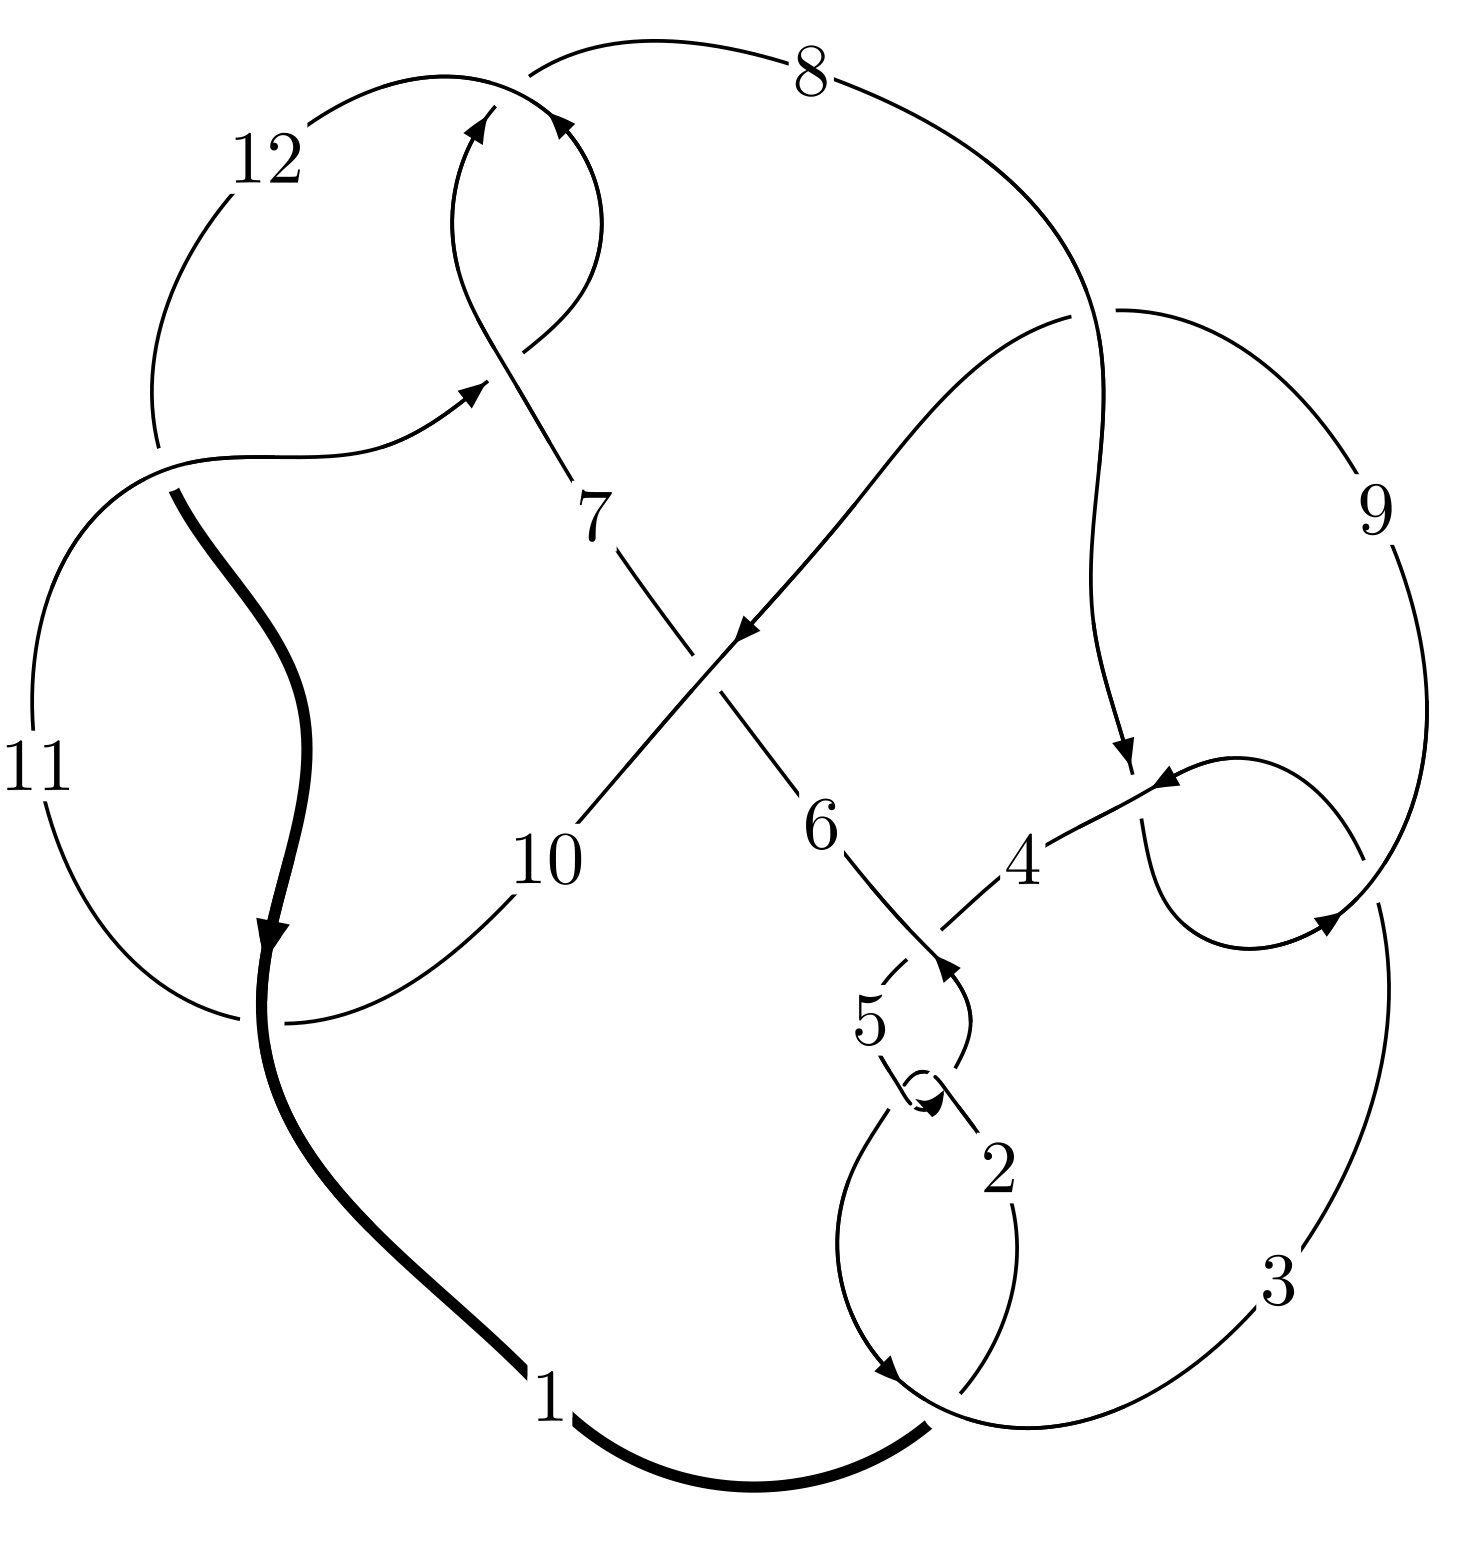
\includegraphics[width=112pt]{../../../GIT/diagram.site/Diagrams/png/976_12a_0175.png}\\
\ \ \ A knot diagram\footnotemark}&
\allowdisplaybreaks
\textbf{Linearized knot diagam} \\
\cline{2-2}
 &
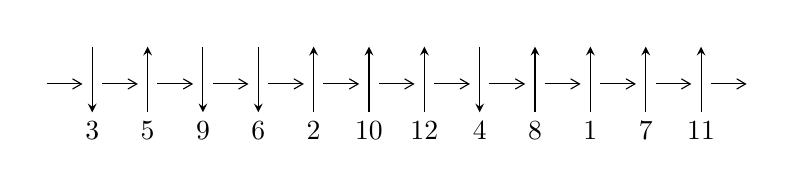
\begin{tikzpicture}[x=20pt, y=17pt]
	% nodes
	\node (C0) at (0, 0) {};
	\node (C1) at (1, 0) {};
	\node (C1U) at (1, +1) {};
	\node (C1D) at (1, -1) {3};

	\node (C2) at (2, 0) {};
	\node (C2U) at (2, +1) {};
	\node (C2D) at (2, -1) {5};

	\node (C3) at (3, 0) {};
	\node (C3U) at (3, +1) {};
	\node (C3D) at (3, -1) {9};

	\node (C4) at (4, 0) {};
	\node (C4U) at (4, +1) {};
	\node (C4D) at (4, -1) {6};

	\node (C5) at (5, 0) {};
	\node (C5U) at (5, +1) {};
	\node (C5D) at (5, -1) {2};

	\node (C6) at (6, 0) {};
	\node (C6U) at (6, +1) {};
	\node (C6D) at (6, -1) {10};

	\node (C7) at (7, 0) {};
	\node (C7U) at (7, +1) {};
	\node (C7D) at (7, -1) {12};

	\node (C8) at (8, 0) {};
	\node (C8U) at (8, +1) {};
	\node (C8D) at (8, -1) {4};

	\node (C9) at (9, 0) {};
	\node (C9U) at (9, +1) {};
	\node (C9D) at (9, -1) {8};

	\node (C10) at (10, 0) {};
	\node (C10U) at (10, +1) {};
	\node (C10D) at (10, -1) {1};

	\node (C11) at (11, 0) {};
	\node (C11U) at (11, +1) {};
	\node (C11D) at (11, -1) {7};

	\node (C12) at (12, 0) {};
	\node (C12U) at (12, +1) {};
	\node (C12D) at (12, -1) {11};
	\node (C13) at (13, 0) {};

	% arrows
	\draw[->,>={angle 60}]
	(C0) edge (C1) (C1) edge (C2) (C2) edge (C3) (C3) edge (C4) (C4) edge (C5) (C5) edge (C6) (C6) edge (C7) (C7) edge (C8) (C8) edge (C9) (C9) edge (C10) (C10) edge (C11) (C11) edge (C12) (C12) edge (C13) ;	\draw[->,>=stealth]
	(C1U) edge (C1D) (C2D) edge (C2U) (C3U) edge (C3D) (C4U) edge (C4D) (C5D) edge (C5U) (C6D) edge (C6U) (C7D) edge (C7U) (C8U) edge (C8D) (C9D) edge (C9U) (C10D) edge (C10U) (C11D) edge (C11U) (C12D) edge (C12U) ;
	\end{tikzpicture} \\
\hhline{~~} \\& 
\textbf{Solving Sequence} \\ \cline{2-2} 
 &
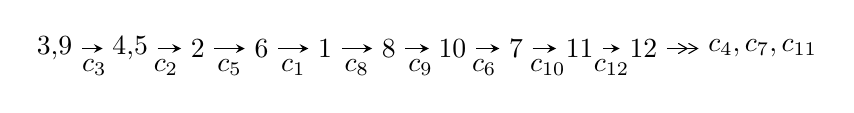
\begin{tikzpicture}[x=23pt, y=7pt]
	% node
	\node (A0) at (-1/8, 0) {3,9};
	\node (A1) at (17/16, 0) {4,5};
	\node (A2) at (17/8, 0) {2};
	\node (A3) at (25/8, 0) {6};
	\node (A4) at (33/8, 0) {1};
	\node (A5) at (41/8, 0) {8};
	\node (A6) at (49/8, 0) {10};
	\node (A7) at (57/8, 0) {7};
	\node (A8) at (65/8, 0) {11};
	\node (A9) at (73/8, 0) {12};
	\node (C1) at (1/2, -1) {$c_{3}$};
	\node (C2) at (13/8, -1) {$c_{2}$};
	\node (C3) at (21/8, -1) {$c_{5}$};
	\node (C4) at (29/8, -1) {$c_{1}$};
	\node (C5) at (37/8, -1) {$c_{8}$};
	\node (C6) at (45/8, -1) {$c_{9}$};
	\node (C7) at (53/8, -1) {$c_{6}$};
	\node (C8) at (61/8, -1) {$c_{10}$};
	\node (C9) at (69/8, -1) {$c_{12}$};
	\node (A10) at (11, 0) {$c_{4},c_{7},c_{11}$};

	% edge
	\draw[->,>=stealth]	
	(A0) edge (A1) (A1) edge (A2) (A2) edge (A3) (A3) edge (A4) (A4) edge (A5) (A5) edge (A6) (A6) edge (A7) (A7) edge (A8) (A8) edge (A9) ;
	\draw[->>,>={angle 60}]	
	(A9) edge (A10);
\end{tikzpicture} \\ 

\end{tabular} \\

\footnotetext{
The image of knot diagram is generated by the software ``\textbf{Draw programme}" developed by Andrew Bartholomew(\url{http://www.layer8.co.uk/maths/draw/index.htm\#Running-draw}), where we modified some parts for our purpose(\url{https://github.com/CATsTAILs/LinksPainter}).
}\phantom \\ \newline 
\centering \textbf{Ideals for irreducible components\footnotemark of $X_{\text{par}}$} 
 
\begin{align*}
I^u_{1}&=\langle 
-3.02409\times10^{165} u^{96}+3.56484\times10^{165} u^{95}+\cdots+6.58858\times10^{165} b-3.79296\times10^{167},\\
\phantom{I^u_{1}}&\phantom{= \langle  }1.29894\times10^{166} u^{96}+1.51856\times10^{166} u^{95}+\cdots+1.31772\times10^{166} a-1.20377\times10^{168},\;u^{97}+u^{96}+\cdots-96 u-64\rangle \\
\\
I^v_{1}&=\langle 
a,\;2 v^5-3 v^4-3 v^3- v^2+5 b+9 v-1,\;v^6- v^5- v^4+3 v^2-2 v+1\rangle \\
\end{align*}
\raggedright * 2 irreducible components of $\dim_{\mathbb{C}}=0$, with total 103 representations.\\
\footnotetext{All coefficients of polynomials are rational numbers. But the coefficients are sometimes approximated in decimal forms when there is not enough margin.}
\newpage
\renewcommand{\arraystretch}{1}
\centering \section*{I. $I^u_{1}= \langle -3.02\times10^{165} u^{96}+3.56\times10^{165} u^{95}+\cdots+6.59\times10^{165} b-3.79\times10^{167},\;1.30\times10^{166} u^{96}+1.52\times10^{166} u^{95}+\cdots+1.32\times10^{166} a-1.20\times10^{168},\;u^{97}+u^{96}+\cdots-96 u-64 \rangle$}
\flushleft \textbf{(i) Arc colorings}\\
\begin{tabular}{m{7pt} m{180pt} m{7pt} m{180pt} }
\flushright $a_{3}=$&$\begin{pmatrix}1\\0\end{pmatrix}$ \\
\flushright $a_{9}=$&$\begin{pmatrix}0\\u\end{pmatrix}$ \\
\flushright $a_{4}=$&$\begin{pmatrix}1\\u^2\end{pmatrix}$ \\
\flushright $a_{5}=$&$\begin{pmatrix}-0.985751 u^{96}-1.15242 u^{95}+\cdots+112.034 u+91.3525\\0.458990 u^{96}-0.541064 u^{95}+\cdots-5.09259 u+57.5687\end{pmatrix}$ \\
\flushright $a_{2}=$&$\begin{pmatrix}-0.884894 u^{96}-1.06215 u^{95}+\cdots+101.503 u+88.1350\\-0.217189 u^{96}+0.134940 u^{95}+\cdots+16.9827 u-39.4811\end{pmatrix}$ \\
\flushright $a_{6}=$&$\begin{pmatrix}-0.884894 u^{96}-1.06215 u^{95}+\cdots+101.503 u+88.1350\\0.991372 u^{96}-0.0100898 u^{95}+\cdots-90.6325 u+28.1367\end{pmatrix}$ \\
\flushright $a_{1}=$&$\begin{pmatrix}-1.10208 u^{96}-0.927210 u^{95}+\cdots+118.486 u+48.6539\\-0.217189 u^{96}+0.134940 u^{95}+\cdots+16.9827 u-39.4811\end{pmatrix}$ \\
\flushright $a_{8}=$&$\begin{pmatrix}u\\u^3+u\end{pmatrix}$ \\
\flushright $a_{10}=$&$\begin{pmatrix}u^3\\u^5+u^3+u\end{pmatrix}$ \\
\flushright $a_{7}=$&$\begin{pmatrix}-0.396152 u^{96}-0.974194 u^{95}+\cdots+50.3059 u+89.0931\\0.711716 u^{96}-0.518934 u^{95}+\cdots-49.1432 u+65.3365\end{pmatrix}$ \\
\flushright $a_{11}=$&$\begin{pmatrix}-0.947269 u^{96}-0.890091 u^{95}+\cdots+88.6821 u+49.4582\\0.0101335 u^{96}+0.113593 u^{95}+\cdots-6.46893 u-26.8412\end{pmatrix}$ \\
\flushright $a_{12}=$&$\begin{pmatrix}-0.764380 u^{96}+0.559446 u^{95}+\cdots+53.8052 u-63.9580\\-1.20457 u^{96}+0.524889 u^{95}+\cdots+75.8592 u-71.8245\end{pmatrix}$\\&\end{tabular}
\flushleft \textbf{(ii) Obstruction class $= -1$}\\~\\
\flushleft \textbf{(iii) Cusp Shapes $= 4.50422 u^{96}+1.68955 u^{95}+\cdots-477.136 u-1.66216$}\\~\\
\newpage\renewcommand{\arraystretch}{1}
\flushleft \textbf{(iv) u-Polynomials at the component}\newline \\
\begin{tabular}{m{50pt}|m{274pt}}
Crossings & \hspace{64pt}u-Polynomials at each crossing \\
\hline $$\begin{aligned}c_{1},c_{4}\end{aligned}$$&$\begin{aligned}
&u^{97}+34 u^{96}+\cdots+11 u-1
\end{aligned}$\\
\hline $$\begin{aligned}c_{2},c_{5}\end{aligned}$$&$\begin{aligned}
&u^{97}+4 u^{96}+\cdots+3 u+1
\end{aligned}$\\
\hline $$\begin{aligned}c_{3},c_{8}\end{aligned}$$&$\begin{aligned}
&u^{97}+u^{96}+\cdots-96 u-64
\end{aligned}$\\
\hline $$\begin{aligned}c_{6}\end{aligned}$$&$\begin{aligned}
&u^{97}+3 u^{96}+\cdots-1136 u-1297
\end{aligned}$\\
\hline $$\begin{aligned}c_{7},c_{11}\end{aligned}$$&$\begin{aligned}
&u^{97}-3 u^{96}+\cdots+4 u-1
\end{aligned}$\\
\hline $$\begin{aligned}c_{9}\end{aligned}$$&$\begin{aligned}
&u^{97}-35 u^{96}+\cdots-52224 u+4096
\end{aligned}$\\
\hline $$\begin{aligned}c_{10},c_{12}\end{aligned}$$&$\begin{aligned}
&u^{97}-31 u^{96}+\cdots-14 u-1
\end{aligned}$\\
\hline
\end{tabular}\\~\\
\newpage\renewcommand{\arraystretch}{1}
\flushleft \textbf{(v) Riley Polynomials at the component}\newline \\
\begin{tabular}{m{50pt}|m{274pt}}
Crossings & \hspace{64pt}Riley Polynomials at each crossing \\
\hline $$\begin{aligned}c_{1},c_{4}\end{aligned}$$&$\begin{aligned}
&y^{97}+62 y^{96}+\cdots+555 y-1
\end{aligned}$\\
\hline $$\begin{aligned}c_{2},c_{5}\end{aligned}$$&$\begin{aligned}
&y^{97}+34 y^{96}+\cdots+11 y-1
\end{aligned}$\\
\hline $$\begin{aligned}c_{3},c_{8}\end{aligned}$$&$\begin{aligned}
&y^{97}+35 y^{96}+\cdots-52224 y-4096
\end{aligned}$\\
\hline $$\begin{aligned}c_{6}\end{aligned}$$&$\begin{aligned}
&y^{97}+13 y^{96}+\cdots-65476470 y-1682209
\end{aligned}$\\
\hline $$\begin{aligned}c_{7},c_{11}\end{aligned}$$&$\begin{aligned}
&y^{97}-31 y^{96}+\cdots-14 y-1
\end{aligned}$\\
\hline $$\begin{aligned}c_{9}\end{aligned}$$&$\begin{aligned}
&y^{97}+43 y^{96}+\cdots-200278016 y-16777216
\end{aligned}$\\
\hline $$\begin{aligned}c_{10},c_{12}\end{aligned}$$&$\begin{aligned}
&y^{97}+73 y^{96}+\cdots+50 y-1
\end{aligned}$\\
\hline
\end{tabular}\\~\\
\newpage\flushleft \textbf{(vi) Complex Volumes and Cusp Shapes}
$$\begin{array}{c|c|c}  
\text{Solutions to }I^u_{1}& \I (\text{vol} + \sqrt{-1}CS) & \text{Cusp shape}\\
 \hline 
\begin{aligned}
u &= -0.559211 + 0.833102 I \\
a &= -2.93598 + 0.85719 I \\
b &= \phantom{-}0.640213 + 0.986388 I\end{aligned}
 & -3.66440 + 1.12900 I & \phantom{-0.000000 } 0 \\ \hline\begin{aligned}
u &= -0.559211 - 0.833102 I \\
a &= -2.93598 - 0.85719 I \\
b &= \phantom{-}0.640213 - 0.986388 I\end{aligned}
 & -3.66440 - 1.12900 I & \phantom{-0.000000 } 0 \\ \hline\begin{aligned}
u &= \phantom{-}0.921624 + 0.348229 I \\
a &= \phantom{-}0.705582 + 0.299295 I \\
b &= -0.703026 + 0.720139 I\end{aligned}
 & \phantom{-}3.36866 + 0.02446 I & \phantom{-0.000000 } 0 \\ \hline\begin{aligned}
u &= \phantom{-}0.921624 - 0.348229 I \\
a &= \phantom{-}0.705582 - 0.299295 I \\
b &= -0.703026 - 0.720139 I\end{aligned}
 & \phantom{-}3.36866 - 0.02446 I & \phantom{-0.000000 } 0 \\ \hline\begin{aligned}
u &= \phantom{-}0.103697 + 0.973816 I \\
a &= \phantom{-}0.806800 + 0.028255 I \\
b &= -0.622905 + 0.069810 I\end{aligned}
 & \phantom{-}1.22652 + 2.27353 I & \phantom{-0.000000 } 0 \\ \hline\begin{aligned}
u &= \phantom{-}0.103697 - 0.973816 I \\
a &= \phantom{-}0.806800 - 0.028255 I \\
b &= -0.622905 - 0.069810 I\end{aligned}
 & \phantom{-}1.22652 - 2.27353 I & \phantom{-0.000000 } 0 \\ \hline\begin{aligned}
u &= \phantom{-}0.617672 + 0.836741 I \\
a &= \phantom{-}0.633968 - 0.472132 I \\
b &= -0.574678 - 1.048600 I\end{aligned}
 & -4.19841 + 2.32705 I & \phantom{-0.000000 } 0 \\ \hline\begin{aligned}
u &= \phantom{-}0.617672 - 0.836741 I \\
a &= \phantom{-}0.633968 + 0.472132 I \\
b &= -0.574678 + 1.048600 I\end{aligned}
 & -4.19841 - 2.32705 I & \phantom{-0.000000 } 0 \\ \hline\begin{aligned}
u &= \phantom{-}0.393076 + 0.966556 I \\
a &= \phantom{-}0.784752 + 0.104315 I \\
b &= -0.665790 + 0.256866 I\end{aligned}
 & \phantom{-}3.71107 - 2.90743 I & \phantom{-0.000000 } 0 \\ \hline\begin{aligned}
u &= \phantom{-}0.393076 - 0.966556 I \\
a &= \phantom{-}0.784752 - 0.104315 I \\
b &= -0.665790 - 0.256866 I\end{aligned}
 & \phantom{-}3.71107 + 2.90743 I & \phantom{-0.000000 } 0\\
 \hline 
 \end{array}$$\newpage$$\begin{array}{c|c|c}  
\text{Solutions to }I^u_{1}& \I (\text{vol} + \sqrt{-1}CS) & \text{Cusp shape}\\
 \hline 
\begin{aligned}
u &= \phantom{-}0.954076 + 0.047302 I \\
a &= \phantom{-}0.678888 + 0.343504 I \\
b &= -0.696044 + 0.825381 I\end{aligned}
 & \phantom{-}0.64837 - 4.98811 I & \phantom{-0.000000 } 0 \\ \hline\begin{aligned}
u &= \phantom{-}0.954076 - 0.047302 I \\
a &= \phantom{-}0.678888 - 0.343504 I \\
b &= -0.696044 - 0.825381 I\end{aligned}
 & \phantom{-}0.64837 + 4.98811 I & \phantom{-0.000000 } 0 \\ \hline\begin{aligned}
u &= -0.645300 + 0.703994 I \\
a &= \phantom{-}1.023660 - 0.910421 I \\
b &= -0.030603 - 0.969352 I\end{aligned}
 & -1.316410 - 0.236436 I & \phantom{-0.000000 } 0 \\ \hline\begin{aligned}
u &= -0.645300 - 0.703994 I \\
a &= \phantom{-}1.023660 + 0.910421 I \\
b &= -0.030603 + 0.969352 I\end{aligned}
 & -1.316410 + 0.236436 I & \phantom{-0.000000 } 0 \\ \hline\begin{aligned}
u &= -0.569710 + 0.879256 I \\
a &= \phantom{-}0.633784 + 0.481988 I \\
b &= -0.560621 + 1.057840 I\end{aligned}
 & -3.50660 + 3.37785 I & \phantom{-0.000000 } 0 \\ \hline\begin{aligned}
u &= -0.569710 - 0.879256 I \\
a &= \phantom{-}0.633784 - 0.481988 I \\
b &= -0.560621 - 1.057840 I\end{aligned}
 & -3.50660 - 3.37785 I & \phantom{-0.000000 } 0 \\ \hline\begin{aligned}
u &= \phantom{-}0.601512 + 0.865138 I \\
a &= -2.72515 - 0.88927 I \\
b &= \phantom{-}0.646669 - 0.998365 I\end{aligned}
 & -4.11264 - 7.12461 I & \phantom{-0.000000 } 0 \\ \hline\begin{aligned}
u &= \phantom{-}0.601512 - 0.865138 I \\
a &= -2.72515 + 0.88927 I \\
b &= \phantom{-}0.646669 + 0.998365 I\end{aligned}
 & -4.11264 + 7.12461 I & \phantom{-0.000000 } 0 \\ \hline\begin{aligned}
u &= -0.926244 + 0.145352 I \\
a &= \phantom{-}0.666759 + 0.369780 I \\
b &= -0.680149 + 0.880890 I\end{aligned}
 & \phantom{-}0.473530 - 0.305894 I & \phantom{-0.000000 } 0 \\ \hline\begin{aligned}
u &= -0.926244 - 0.145352 I \\
a &= \phantom{-}0.666759 - 0.369780 I \\
b &= -0.680149 - 0.880890 I\end{aligned}
 & \phantom{-}0.473530 + 0.305894 I & \phantom{-0.000000 } 0\\
 \hline 
 \end{array}$$\newpage$$\begin{array}{c|c|c}  
\text{Solutions to }I^u_{1}& \I (\text{vol} + \sqrt{-1}CS) & \text{Cusp shape}\\
 \hline 
\begin{aligned}
u &= -0.951056 + 0.474035 I \\
a &= \phantom{-}0.636506 + 0.403254 I \\
b &= -0.673700 + 0.969389 I\end{aligned}
 & \phantom{-}2.60981 - 5.33424 I & \phantom{-0.000000 } 0 \\ \hline\begin{aligned}
u &= -0.951056 - 0.474035 I \\
a &= \phantom{-}0.636506 - 0.403254 I \\
b &= -0.673700 - 0.969389 I\end{aligned}
 & \phantom{-}2.60981 + 5.33424 I & \phantom{-0.000000 } 0 \\ \hline\begin{aligned}
u &= -0.909599 + 0.577057 I \\
a &= \phantom{-}0.715967 - 0.254923 I \\
b &= -0.728203 - 0.626828 I\end{aligned}
 & -2.48877 + 0.51312 I & \phantom{-0.000000 } 0 \\ \hline\begin{aligned}
u &= -0.909599 - 0.577057 I \\
a &= \phantom{-}0.715967 + 0.254923 I \\
b &= -0.728203 + 0.626828 I\end{aligned}
 & -2.48877 - 0.51312 I & \phantom{-0.000000 } 0 \\ \hline\begin{aligned}
u &= -0.808800 + 0.713714 I \\
a &= \phantom{-}0.92259 - 1.12481 I \\
b &= \phantom{-}0.038627 - 1.049570 I\end{aligned}
 & -7.27155 - 4.70566 I & \phantom{-0.000000 } 0 \\ \hline\begin{aligned}
u &= -0.808800 - 0.713714 I \\
a &= \phantom{-}0.92259 + 1.12481 I \\
b &= \phantom{-}0.038627 + 1.049570 I\end{aligned}
 & -7.27155 + 4.70566 I & \phantom{-0.000000 } 0 \\ \hline\begin{aligned}
u &= \phantom{-}0.681205 + 0.843165 I \\
a &= \phantom{-}0.852242 + 0.924197 I \\
b &= -0.064983 + 1.054230 I\end{aligned}
 & -4.00994 - 2.62127 I & \phantom{-0.000000 } 0 \\ \hline\begin{aligned}
u &= \phantom{-}0.681205 - 0.843165 I \\
a &= \phantom{-}0.852242 - 0.924197 I \\
b &= -0.064983 - 1.054230 I\end{aligned}
 & -4.00994 + 2.62127 I & \phantom{-0.000000 } 0 \\ \hline\begin{aligned}
u &= \phantom{-}0.739984 + 0.538074 I \\
a &= \phantom{-}0.652275 - 0.428907 I \\
b &= -0.617449 - 0.977470 I\end{aligned}
 & -0.76408 + 3.26264 I & \phantom{-0.000000 } 0 \\ \hline\begin{aligned}
u &= \phantom{-}0.739984 - 0.538074 I \\
a &= \phantom{-}0.652275 + 0.428907 I \\
b &= -0.617449 + 0.977470 I\end{aligned}
 & -0.76408 - 3.26264 I & \phantom{-0.000000 } 0\\
 \hline 
 \end{array}$$\newpage$$\begin{array}{c|c|c}  
\text{Solutions to }I^u_{1}& \I (\text{vol} + \sqrt{-1}CS) & \text{Cusp shape}\\
 \hline 
\begin{aligned}
u &= \phantom{-}0.802343 + 0.748909 I \\
a &= \phantom{-}0.889988 + 1.090280 I \\
b &= \phantom{-}0.021091 + 1.059600 I\end{aligned}
 & -7.92238 - 1.15791 I & \phantom{-0.000000 } 0 \\ \hline\begin{aligned}
u &= \phantom{-}0.802343 - 0.748909 I \\
a &= \phantom{-}0.889988 - 1.090280 I \\
b &= \phantom{-}0.021091 - 1.059600 I\end{aligned}
 & -7.92238 + 1.15791 I & \phantom{-0.000000 } 0 \\ \hline\begin{aligned}
u &= -0.503977 + 0.742800 I \\
a &= \phantom{-}0.12148 + 1.78100 I \\
b &= \phantom{-}0.639777 - 0.633736 I\end{aligned}
 & -3.04156 + 2.02850 I & \phantom{-}4.00000 - 3.93778 I \\ \hline\begin{aligned}
u &= -0.503977 - 0.742800 I \\
a &= \phantom{-}0.12148 - 1.78100 I \\
b &= \phantom{-}0.639777 + 0.633736 I\end{aligned}
 & -3.04156 - 2.02850 I & \phantom{-}4.00000 + 3.93778 I \\ \hline\begin{aligned}
u &= \phantom{-}0.967362 + 0.550103 I \\
a &= \phantom{-}0.704293 + 0.259773 I \\
b &= -0.746470 + 0.647655 I\end{aligned}
 & -1.70048 + 5.14403 I & \phantom{-0.000000 } 0 \\ \hline\begin{aligned}
u &= \phantom{-}0.967362 - 0.550103 I \\
a &= \phantom{-}0.704293 - 0.259773 I \\
b &= -0.746470 - 0.647655 I\end{aligned}
 & -1.70048 - 5.14403 I & \phantom{-0.000000 } 0 \\ \hline\begin{aligned}
u &= -0.590695 + 0.945576 I \\
a &= \phantom{-}0.756916 - 0.148066 I \\
b &= -0.715182 - 0.368711 I\end{aligned}
 & -2.29120 + 2.48545 I & \phantom{-0.000000 } 0 \\ \hline\begin{aligned}
u &= -0.590695 - 0.945576 I \\
a &= \phantom{-}0.756916 + 0.148066 I \\
b &= -0.715182 + 0.368711 I\end{aligned}
 & -2.29120 - 2.48545 I & \phantom{-0.000000 } 0 \\ \hline\begin{aligned}
u &= -0.614372 + 0.936095 I \\
a &= \phantom{-}0.787074 - 0.853524 I \\
b &= -0.120816 - 1.078960 I\end{aligned}
 & -0.63114 + 5.15568 I & \phantom{-0.000000 } 0 \\ \hline\begin{aligned}
u &= -0.614372 - 0.936095 I \\
a &= \phantom{-}0.787074 + 0.853524 I \\
b &= -0.120816 + 1.078960 I\end{aligned}
 & -0.63114 - 5.15568 I & \phantom{-0.000000 } 0\\
 \hline 
 \end{array}$$\newpage$$\begin{array}{c|c|c}  
\text{Solutions to }I^u_{1}& \I (\text{vol} + \sqrt{-1}CS) & \text{Cusp shape}\\
 \hline 
\begin{aligned}
u &= \phantom{-}0.080865 + 1.133620 I \\
a &= -1.62986 - 1.10490 I \\
b &= \phantom{-}0.752817 + 0.826084 I\end{aligned}
 & \phantom{-}4.36765 + 1.71081 I & \phantom{-0.000000 } 0 \\ \hline\begin{aligned}
u &= \phantom{-}0.080865 - 1.133620 I \\
a &= -1.62986 + 1.10490 I \\
b &= \phantom{-}0.752817 - 0.826084 I\end{aligned}
 & \phantom{-}4.36765 - 1.71081 I & \phantom{-0.000000 } 0 \\ \hline\begin{aligned}
u &= \phantom{-}0.070502 + 0.857380 I \\
a &= \phantom{-}0.729488 + 0.578116 I \\
b &= -0.371245 + 1.016130 I\end{aligned}
 & -1.54806 - 5.69625 I & \phantom{-}5.02059 + 7.78118 I \\ \hline\begin{aligned}
u &= \phantom{-}0.070502 - 0.857380 I \\
a &= \phantom{-}0.729488 - 0.578116 I \\
b &= -0.371245 - 1.016130 I\end{aligned}
 & -1.54806 + 5.69625 I & \phantom{-}5.02059 - 7.78118 I \\ \hline\begin{aligned}
u &= -0.216302 + 0.821989 I \\
a &= \phantom{-}0.777283 - 0.606819 I \\
b &= -0.313813 - 0.989855 I\end{aligned}
 & -1.89002 + 0.62557 I & \phantom{-}3.27682 - 2.54234 I \\ \hline\begin{aligned}
u &= -0.216302 - 0.821989 I \\
a &= \phantom{-}0.777283 + 0.606819 I \\
b &= -0.313813 + 0.989855 I\end{aligned}
 & -1.89002 - 0.62557 I & \phantom{-}3.27682 + 2.54234 I \\ \hline\begin{aligned}
u &= \phantom{-}0.572877 + 1.000360 I \\
a &= \phantom{-}0.750719 + 0.135692 I \\
b &= -0.735264 + 0.342685 I\end{aligned}
 & -1.45728 - 8.16426 I & \phantom{-0.000000 } 0 \\ \hline\begin{aligned}
u &= \phantom{-}0.572877 - 1.000360 I \\
a &= \phantom{-}0.750719 - 0.135692 I \\
b &= -0.735264 - 0.342685 I\end{aligned}
 & -1.45728 + 8.16426 I & \phantom{-0.000000 } 0 \\ \hline\begin{aligned}
u &= \phantom{-}0.959758 + 0.642441 I \\
a &= \phantom{-}0.620834 - 0.418859 I \\
b &= -0.668914 - 1.012510 I\end{aligned}
 & -3.62554 + 4.84764 I & \phantom{-0.000000 } 0 \\ \hline\begin{aligned}
u &= \phantom{-}0.959758 - 0.642441 I \\
a &= \phantom{-}0.620834 + 0.418859 I \\
b &= -0.668914 + 1.012510 I\end{aligned}
 & -3.62554 - 4.84764 I & \phantom{-0.000000 } 0\\
 \hline 
 \end{array}$$\newpage$$\begin{array}{c|c|c}  
\text{Solutions to }I^u_{1}& \I (\text{vol} + \sqrt{-1}CS) & \text{Cusp shape}\\
 \hline 
\begin{aligned}
u &= -0.181422 + 1.152130 I \\
a &= -2.08238 - 0.57032 I \\
b &= \phantom{-}0.740928 + 0.901905 I\end{aligned}
 & \phantom{-}4.13850 + 3.94348 I & \phantom{-0.000000 } 0 \\ \hline\begin{aligned}
u &= -0.181422 - 1.152130 I \\
a &= -2.08238 + 0.57032 I \\
b &= \phantom{-}0.740928 - 0.901905 I\end{aligned}
 & \phantom{-}4.13850 - 3.94348 I & \phantom{-0.000000 } 0 \\ \hline\begin{aligned}
u &= \phantom{-}0.428081 + 1.088840 I \\
a &= -0.80049 - 1.24984 I \\
b &= \phantom{-}0.772564 + 0.710004 I\end{aligned}
 & \phantom{-}4.18113 + 0.71587 I & \phantom{-0.000000 } 0 \\ \hline\begin{aligned}
u &= \phantom{-}0.428081 - 1.088840 I \\
a &= -0.80049 + 1.24984 I \\
b &= \phantom{-}0.772564 - 0.710004 I\end{aligned}
 & \phantom{-}4.18113 - 0.71587 I & \phantom{-0.000000 } 0 \\ \hline\begin{aligned}
u &= -0.563061 + 1.032860 I \\
a &= -0.503416 + 1.194440 I \\
b &= \phantom{-}0.773133 - 0.653958 I\end{aligned}
 & \phantom{-}1.84211 + 2.97512 I & \phantom{-0.000000 } 0 \\ \hline\begin{aligned}
u &= -0.563061 - 1.032860 I \\
a &= -0.503416 - 1.194440 I \\
b &= \phantom{-}0.773133 + 0.653958 I\end{aligned}
 & \phantom{-}1.84211 - 2.97512 I & \phantom{-0.000000 } 0 \\ \hline\begin{aligned}
u &= -1.002940 + 0.626538 I \\
a &= \phantom{-}0.618218 + 0.413528 I \\
b &= -0.680442 + 1.010310 I\end{aligned}
 & -2.78079 - 10.59270 I & \phantom{-0.000000 } 0 \\ \hline\begin{aligned}
u &= -1.002940 - 0.626538 I \\
a &= \phantom{-}0.618218 - 0.413528 I \\
b &= -0.680442 - 1.010310 I\end{aligned}
 & -2.78079 + 10.59270 I & \phantom{-0.000000 } 0 \\ \hline\begin{aligned}
u &= \phantom{-}0.411216 + 0.705558 I \\
a &= \phantom{-}0.10856 - 2.30048 I \\
b &= \phantom{-}0.613326 + 0.678658 I\end{aligned}
 & -2.71127 + 3.87377 I & \phantom{-}5.00270 - 0.93534 I \\ \hline\begin{aligned}
u &= \phantom{-}0.411216 - 0.705558 I \\
a &= \phantom{-}0.10856 + 2.30048 I \\
b &= \phantom{-}0.613326 - 0.678658 I\end{aligned}
 & -2.71127 - 3.87377 I & \phantom{-}5.00270 + 0.93534 I\\
 \hline 
 \end{array}$$\newpage$$\begin{array}{c|c|c}  
\text{Solutions to }I^u_{1}& \I (\text{vol} + \sqrt{-1}CS) & \text{Cusp shape}\\
 \hline 
\begin{aligned}
u &= -0.322378 + 0.730346 I \\
a &= \phantom{-}0.680499 + 0.494589 I \\
b &= -0.502195 + 1.006730 I\end{aligned}
 & \phantom{-}1.62089 - 1.29744 I & \phantom{-}10.04280 - 2.09415 I \\ \hline\begin{aligned}
u &= -0.322378 - 0.730346 I \\
a &= \phantom{-}0.680499 - 0.494589 I \\
b &= -0.502195 - 1.006730 I\end{aligned}
 & \phantom{-}1.62089 + 1.29744 I & \phantom{-}10.04280 + 2.09415 I \\ \hline\begin{aligned}
u &= -0.528635 + 1.079550 I \\
a &= -2.29831 + 0.32828 I \\
b &= \phantom{-}0.704089 + 0.988971 I\end{aligned}
 & \phantom{-}3.33114 + 4.88044 I & \phantom{-0.000000 } 0 \\ \hline\begin{aligned}
u &= -0.528635 - 1.079550 I \\
a &= -2.29831 - 0.32828 I \\
b &= \phantom{-}0.704089 - 0.988971 I\end{aligned}
 & \phantom{-}3.33114 - 4.88044 I & \phantom{-0.000000 } 0 \\ \hline\begin{aligned}
u &= \phantom{-}0.722689 + 0.970599 I \\
a &= \phantom{-}0.741299 + 0.921828 I \\
b &= -0.083570 + 1.119970 I\end{aligned}
 & -7.22715 - 4.57605 I & \phantom{-0.000000 } 0 \\ \hline\begin{aligned}
u &= \phantom{-}0.722689 - 0.970599 I \\
a &= \phantom{-}0.741299 - 0.921828 I \\
b &= -0.083570 - 1.119970 I\end{aligned}
 & -7.22715 + 4.57605 I & \phantom{-0.000000 } 0 \\ \hline\begin{aligned}
u &= -0.358259 + 0.688871 I \\
a &= \phantom{-}0.879547 - 0.142406 I \\
b &= -0.452675 - 0.326769 I\end{aligned}
 & \phantom{-}0.242270 + 1.201440 I & \phantom{-}3.56976 - 5.11662 I \\ \hline\begin{aligned}
u &= -0.358259 - 0.688871 I \\
a &= \phantom{-}0.879547 + 0.142406 I \\
b &= -0.452675 + 0.326769 I\end{aligned}
 & \phantom{-}0.242270 - 1.201440 I & \phantom{-}3.56976 + 5.11662 I \\ \hline\begin{aligned}
u &= -0.709964 + 0.998104 I \\
a &= \phantom{-}0.727209 - 0.906231 I \\
b &= -0.095370 - 1.127510 I\end{aligned}
 & -6.38097 + 10.41820 I & \phantom{-0.000000 } 0 \\ \hline\begin{aligned}
u &= -0.709964 - 0.998104 I \\
a &= \phantom{-}0.727209 + 0.906231 I \\
b &= -0.095370 + 1.127510 I\end{aligned}
 & -6.38097 - 10.41820 I & \phantom{-0.000000 } 0\\
 \hline 
 \end{array}$$\newpage$$\begin{array}{c|c|c}  
\text{Solutions to }I^u_{1}& \I (\text{vol} + \sqrt{-1}CS) & \text{Cusp shape}\\
 \hline 
\begin{aligned}
u &= \phantom{-}0.638479 + 1.052860 I \\
a &= -2.22261 - 0.60109 I \\
b &= \phantom{-}0.692459 - 1.015440 I\end{aligned}
 & \phantom{-}0.75759 - 8.53408 I & \phantom{-0.000000 } 0 \\ \hline\begin{aligned}
u &= \phantom{-}0.638479 - 1.052860 I \\
a &= -2.22261 + 0.60109 I \\
b &= \phantom{-}0.692459 + 1.015440 I\end{aligned}
 & \phantom{-}0.75759 + 8.53408 I & \phantom{-0.000000 } 0 \\ \hline\begin{aligned}
u &= -0.128439 + 1.243580 I \\
a &= -1.41997 + 0.92023 I \\
b &= \phantom{-}0.789225 - 0.821137 I\end{aligned}
 & \phantom{-}5.72877 + 3.22175 I & \phantom{-0.000000 } 0 \\ \hline\begin{aligned}
u &= -0.128439 - 1.243580 I \\
a &= -1.41997 - 0.92023 I \\
b &= \phantom{-}0.789225 + 0.821137 I\end{aligned}
 & \phantom{-}5.72877 - 3.22175 I & \phantom{-0.000000 } 0 \\ \hline\begin{aligned}
u &= \phantom{-}0.045313 + 1.258340 I \\
a &= -1.69439 + 0.69129 I \\
b &= \phantom{-}0.779135 - 0.871630 I\end{aligned}
 & \phantom{-}9.43059 - 2.92424 I & \phantom{-0.000000 } 0 \\ \hline\begin{aligned}
u &= \phantom{-}0.045313 - 1.258340 I \\
a &= -1.69439 - 0.69129 I \\
b &= \phantom{-}0.779135 + 0.871630 I\end{aligned}
 & \phantom{-}9.43059 + 2.92424 I & \phantom{-0.000000 } 0 \\ \hline\begin{aligned}
u &= \phantom{-}0.211932 + 1.248480 I \\
a &= -1.90337 + 0.41008 I \\
b &= \phantom{-}0.764919 - 0.916036 I\end{aligned}
 & \phantom{-}5.44080 - 9.05611 I & \phantom{-0.000000 } 0 \\ \hline\begin{aligned}
u &= \phantom{-}0.211932 - 1.248480 I \\
a &= -1.90337 - 0.41008 I \\
b &= \phantom{-}0.764919 + 0.916036 I\end{aligned}
 & \phantom{-}5.44080 + 9.05611 I & \phantom{-0.000000 } 0 \\ \hline\begin{aligned}
u &= \phantom{-}0.605096 + 1.135060 I \\
a &= -0.565397 - 1.012220 I \\
b &= \phantom{-}0.815794 + 0.657405 I\end{aligned}
 & \phantom{-}5.78450 - 5.48770 I & \phantom{-0.000000 } 0 \\ \hline\begin{aligned}
u &= \phantom{-}0.605096 - 1.135060 I \\
a &= -0.565397 + 1.012220 I \\
b &= \phantom{-}0.815794 - 0.657405 I\end{aligned}
 & \phantom{-}5.78450 + 5.48770 I & \phantom{-0.000000 } 0\\
 \hline 
 \end{array}$$\newpage$$\begin{array}{c|c|c}  
\text{Solutions to }I^u_{1}& \I (\text{vol} + \sqrt{-1}CS) & \text{Cusp shape}\\
 \hline 
\begin{aligned}
u &= -0.701626 + 1.089850 I \\
a &= -0.417547 + 0.958298 I \\
b &= \phantom{-}0.819456 - 0.616638 I\end{aligned}
 & -0.89248 + 5.41548 I & \phantom{-0.000000 } 0 \\ \hline\begin{aligned}
u &= -0.701626 - 1.089850 I \\
a &= -0.417547 - 0.958298 I \\
b &= \phantom{-}0.819456 + 0.616638 I\end{aligned}
 & -0.89248 - 5.41548 I & \phantom{-0.000000 } 0 \\ \hline\begin{aligned}
u &= \phantom{-}0.587493 + 0.354318 I \\
a &= \phantom{-}1.107100 - 0.364526 I \\
b &= \phantom{-}0.334542 + 0.368918 I\end{aligned}
 & -2.95310 + 3.72297 I & \phantom{-}0.94420 - 2.07309 I \\ \hline\begin{aligned}
u &= \phantom{-}0.587493 - 0.354318 I \\
a &= \phantom{-}1.107100 + 0.364526 I \\
b &= \phantom{-}0.334542 - 0.368918 I\end{aligned}
 & -2.95310 - 3.72297 I & \phantom{-}0.94420 + 2.07309 I \\ \hline\begin{aligned}
u &= -0.669813 + 1.133570 I \\
a &= -2.03613 + 0.55346 I \\
b &= \phantom{-}0.711185 + 1.026810 I\end{aligned}
 & \phantom{-}4.66603 + 11.22230 I & \phantom{-0.000000 } 0 \\ \hline\begin{aligned}
u &= -0.669813 - 1.133570 I \\
a &= -2.03613 - 0.55346 I \\
b &= \phantom{-}0.711185 - 1.026810 I\end{aligned}
 & \phantom{-}4.66603 - 11.22230 I & \phantom{-0.000000 } 0 \\ \hline\begin{aligned}
u &= \phantom{-}0.748378 + 1.095500 I \\
a &= -1.99348 - 0.72388 I \\
b &= \phantom{-}0.698362 - 1.044580 I\end{aligned}
 & -2.18107 - 11.11030 I & \phantom{-0.000000 } 0 \\ \hline\begin{aligned}
u &= \phantom{-}0.748378 - 1.095500 I \\
a &= -1.99348 + 0.72388 I \\
b &= \phantom{-}0.698362 + 1.044580 I\end{aligned}
 & -2.18107 + 11.11030 I & \phantom{-0.000000 } 0 \\ \hline\begin{aligned}
u &= \phantom{-}0.711168 + 1.121910 I \\
a &= -0.443302 - 0.920203 I \\
b &= \phantom{-}0.831954 + 0.620163 I\end{aligned}
 & \phantom{-}0.09597 - 11.25780 I & \phantom{-0.000000 } 0 \\ \hline\begin{aligned}
u &= \phantom{-}0.711168 - 1.121910 I \\
a &= -0.443302 + 0.920203 I \\
b &= \phantom{-}0.831954 - 0.620163 I\end{aligned}
 & \phantom{-}0.09597 + 11.25780 I & \phantom{-0.000000 } 0\\
 \hline 
 \end{array}$$\newpage$$\begin{array}{c|c|c}  
\text{Solutions to }I^u_{1}& \I (\text{vol} + \sqrt{-1}CS) & \text{Cusp shape}\\
 \hline 
\begin{aligned}
u &= -0.536075 + 0.400740 I \\
a &= \phantom{-}1.39980 + 0.27771 I \\
b &= \phantom{-}0.260700 - 0.482970 I\end{aligned}
 & -3.25787 + 1.87409 I & -0.41579 - 4.30108 I \\ \hline\begin{aligned}
u &= -0.536075 - 0.400740 I \\
a &= \phantom{-}1.39980 - 0.27771 I \\
b &= \phantom{-}0.260700 + 0.482970 I\end{aligned}
 & -3.25787 - 1.87409 I & -0.41579 + 4.30108 I \\ \hline\begin{aligned}
u &= -0.757737 + 1.120540 I \\
a &= -1.94603 + 0.70259 I \\
b &= \phantom{-}0.704135 + 1.047940 I\end{aligned}
 & -1.1974 + 17.0067 I & \phantom{-0.000000 } 0 \\ \hline\begin{aligned}
u &= -0.757737 - 1.120540 I \\
a &= -1.94603 - 0.70259 I \\
b &= \phantom{-}0.704135 - 1.047940 I\end{aligned}
 & -1.1974 - 17.0067 I & \phantom{-0.000000 } 0 \\ \hline\begin{aligned}
u &= -0.548785 + 0.324950 I \\
a &= \phantom{-}0.777437 - 0.349360 I \\
b &= -0.540827 - 0.732581 I\end{aligned}
 & \phantom{-}0.11105 + 1.45554 I & -0.54843 - 3.22563 I \\ \hline\begin{aligned}
u &= -0.548785 - 0.324950 I \\
a &= \phantom{-}0.777437 + 0.349360 I \\
b &= -0.540827 + 0.732581 I\end{aligned}
 & \phantom{-}0.11105 - 1.45554 I & -0.54843 + 3.22563 I \\ \hline\begin{aligned}
u &= \phantom{-}0.456001\phantom{ +0.000000I} \\
a &= \phantom{-}0.952554\phantom{ +0.000000I} \\
b &= \phantom{-}0.199661\phantom{ +0.000000I}\end{aligned}
 & \phantom{-}1.36800\phantom{ +0.000000I} & \phantom{-}6.81850\phantom{ +0.000000I}\\
 \hline 
 \end{array}$$\newpage\newpage\renewcommand{\arraystretch}{1}
\centering \section*{II. $I^v_{1}= \langle a,\;2 v^5-3 v^4-3 v^3- v^2+5 b+9 v-1,\;v^6- v^5- v^4+3 v^2-2 v+1 \rangle$}
\flushleft \textbf{(i) Arc colorings}\\
\begin{tabular}{m{7pt} m{180pt} m{7pt} m{180pt} }
\flushright $a_{3}=$&$\begin{pmatrix}1\\0\end{pmatrix}$ \\
\flushright $a_{9}=$&$\begin{pmatrix}v\\0\end{pmatrix}$ \\
\flushright $a_{4}=$&$\begin{pmatrix}1\\0\end{pmatrix}$ \\
\flushright $a_{5}=$&$\begin{pmatrix}0\\-\frac{2}{5} v^5+\frac{3}{5} v^4+\cdots-\frac{9}{5} v+\frac{1}{5}\end{pmatrix}$ \\
\flushright $a_{2}=$&$\begin{pmatrix}1\\\frac{2}{5} v^5-\frac{3}{5} v^4+\cdots+\frac{9}{5} v-\frac{6}{5}\end{pmatrix}$ \\
\flushright $a_{6}=$&$\begin{pmatrix}-\frac{2}{5} v^5+\frac{3}{5} v^4+\cdots-\frac{9}{5} v+\frac{1}{5}\\-\frac{2}{5} v^5+\frac{3}{5} v^4+\cdots-\frac{9}{5} v+\frac{6}{5}\end{pmatrix}$ \\
\flushright $a_{1}=$&$\begin{pmatrix}\frac{2}{5} v^5-\frac{3}{5} v^4+\cdots+\frac{9}{5} v-\frac{1}{5}\\\frac{2}{5} v^5-\frac{3}{5} v^4+\cdots+\frac{9}{5} v-\frac{6}{5}\end{pmatrix}$ \\
\flushright $a_{8}=$&$\begin{pmatrix}v\\0\end{pmatrix}$ \\
\flushright $a_{10}=$&$\begin{pmatrix}v\\0\end{pmatrix}$ \\
\flushright $a_{7}=$&$\begin{pmatrix}v^4- v\\-\frac{2}{5} v^5+\frac{3}{5} v^4+\cdots-\frac{9}{5} v+\frac{6}{5}\end{pmatrix}$ \\
\flushright $a_{11}=$&$\begin{pmatrix}2 v\\-\frac{1}{5} v^5-\frac{1}{5} v^4+\cdots+\frac{3}{5} v-\frac{2}{5}\end{pmatrix}$ \\
\flushright $a_{12}=$&$\begin{pmatrix}\frac{6}{5} v^5+\frac{1}{5} v^4+\cdots+\frac{17}{5} v-\frac{3}{5}\\\frac{2}{5} v^5-\frac{3}{5} v^4+\cdots+\frac{9}{5} v-\frac{6}{5}\end{pmatrix}$\\&\end{tabular}
\flushleft \textbf{(ii) Obstruction class $= 1$}\\~\\
\flushleft \textbf{(iii) Cusp Shapes $= -\frac{14}{5} v^5+\frac{21}{5} v^4+\frac{11}{5} v^3+\frac{2}{5} v^2-\frac{58}{5} v+\frac{47}{5}$}\\~\\
\newpage\renewcommand{\arraystretch}{1}
\flushleft \textbf{(iv) u-Polynomials at the component}\newline \\
\begin{tabular}{m{50pt}|m{274pt}}
Crossings & \hspace{64pt}u-Polynomials at each crossing \\
\hline $$\begin{aligned}c_{1},c_{4},c_{5}\end{aligned}$$&$\begin{aligned}
&(u^2- u+1)^3
\end{aligned}$\\
\hline $$\begin{aligned}c_{2}\end{aligned}$$&$\begin{aligned}
&(u^2+u+1)^3
\end{aligned}$\\
\hline $$\begin{aligned}c_{3},c_{8},c_{9}\end{aligned}$$&$\begin{aligned}
&u^6
\end{aligned}$\\
\hline $$\begin{aligned}c_{6},c_{10}\end{aligned}$$&$\begin{aligned}
&(u^3+u^2+2 u+1)^2
\end{aligned}$\\
\hline $$\begin{aligned}c_{7}\end{aligned}$$&$\begin{aligned}
&(u^3- u^2+1)^2
\end{aligned}$\\
\hline $$\begin{aligned}c_{11}\end{aligned}$$&$\begin{aligned}
&(u^3+u^2-1)^2
\end{aligned}$\\
\hline $$\begin{aligned}c_{12}\end{aligned}$$&$\begin{aligned}
&(u^3- u^2+2 u-1)^2
\end{aligned}$\\
\hline
\end{tabular}\\~\\
\newpage\renewcommand{\arraystretch}{1}
\flushleft \textbf{(v) Riley Polynomials at the component}\newline \\
\begin{tabular}{m{50pt}|m{274pt}}
Crossings & \hspace{64pt}Riley Polynomials at each crossing \\
\hline $$\begin{aligned}c_{1},c_{2},c_{4}\\c_{5}\end{aligned}$$&$\begin{aligned}
&(y^2+y+1)^3
\end{aligned}$\\
\hline $$\begin{aligned}c_{3},c_{8},c_{9}\end{aligned}$$&$\begin{aligned}
&y^6
\end{aligned}$\\
\hline $$\begin{aligned}c_{6},c_{10},c_{12}\end{aligned}$$&$\begin{aligned}
&(y^3+3 y^2+2 y-1)^2
\end{aligned}$\\
\hline $$\begin{aligned}c_{7},c_{11}\end{aligned}$$&$\begin{aligned}
&(y^3- y^2+2 y-1)^2
\end{aligned}$\\
\hline
\end{tabular}\\~\\
\newpage\flushleft \textbf{(vi) Complex Volumes and Cusp Shapes}
$$\begin{array}{c|c|c}  
\text{Solutions to }I^v_{1}& \I (\text{vol} + \sqrt{-1}CS) & \text{Cusp shape}\\
 \hline 
\begin{aligned}
v &= -1.024480 + 0.839835 I \\
a &= \phantom{-0.000000 } 0 \\
b &= -0.500000 - 0.866025 I\end{aligned}
 & -3.02413 + 4.85801 I & \phantom{-}0.94625 - 7.60556 I \\ \hline\begin{aligned}
v &= -1.024480 - 0.839835 I \\
a &= \phantom{-0.000000 } 0 \\
b &= -0.500000 + 0.866025 I\end{aligned}
 & -3.02413 - 4.85801 I & \phantom{-}0.94625 + 7.60556 I \\ \hline\begin{aligned}
v &= \phantom{-}1.239560 + 0.467306 I \\
a &= \phantom{-0.000000 } 0 \\
b &= -0.500000 + 0.866025 I\end{aligned}
 & -3.02413 + 0.79824 I & \phantom{-}2.23639 + 1.26697 I \\ \hline\begin{aligned}
v &= \phantom{-}1.239560 - 0.467306 I \\
a &= \phantom{-0.000000 } 0 \\
b &= -0.500000 - 0.866025 I\end{aligned}
 & -3.02413 - 0.79824 I & \phantom{-}2.23639 - 1.26697 I \\ \hline\begin{aligned}
v &= \phantom{-}0.284920 + 0.493496 I \\
a &= \phantom{-0.000000 } 0 \\
b &= -0.500000 - 0.866025 I\end{aligned}
 & \phantom{-}1.11345 + 2.02988 I & \phantom{-}5.31735 - 5.84990 I \\ \hline\begin{aligned}
v &= \phantom{-}0.284920 - 0.493496 I \\
a &= \phantom{-0.000000 } 0 \\
b &= -0.500000 + 0.866025 I\end{aligned}
 & \phantom{-}1.11345 - 2.02988 I & \phantom{-}5.31735 + 5.84990 I\\
 \hline 
 \end{array}$$\newpage
\newpage\renewcommand{\arraystretch}{1}
\centering \section*{ III. u-Polynomials}
\begin{tabular}{m{50pt}|m{274pt}}
Crossings & \hspace{64pt}u-Polynomials at each crossing \\
\hline $$\begin{aligned}c_{1},c_{4}\end{aligned}$$&$\begin{aligned}
&((u^2- u+1)^3)(u^{97}+34 u^{96}+\cdots+11 u-1)
\end{aligned}$\\
\hline $$\begin{aligned}c_{2}\end{aligned}$$&$\begin{aligned}
&((u^2+u+1)^3)(u^{97}+4 u^{96}+\cdots+3 u+1)
\end{aligned}$\\
\hline $$\begin{aligned}c_{3},c_{8}\end{aligned}$$&$\begin{aligned}
&u^6(u^{97}+u^{96}+\cdots-96 u-64)
\end{aligned}$\\
\hline $$\begin{aligned}c_{5}\end{aligned}$$&$\begin{aligned}
&((u^2- u+1)^3)(u^{97}+4 u^{96}+\cdots+3 u+1)
\end{aligned}$\\
\hline $$\begin{aligned}c_{6}\end{aligned}$$&$\begin{aligned}
&((u^3+u^2+2 u+1)^2)(u^{97}+3 u^{96}+\cdots-1136 u-1297)
\end{aligned}$\\
\hline $$\begin{aligned}c_{7}\end{aligned}$$&$\begin{aligned}
&((u^3- u^2+1)^2)(u^{97}-3 u^{96}+\cdots+4 u-1)
\end{aligned}$\\
\hline $$\begin{aligned}c_{9}\end{aligned}$$&$\begin{aligned}
&u^6(u^{97}-35 u^{96}+\cdots-52224 u+4096)
\end{aligned}$\\
\hline $$\begin{aligned}c_{10}\end{aligned}$$&$\begin{aligned}
&((u^3+u^2+2 u+1)^2)(u^{97}-31 u^{96}+\cdots-14 u-1)
\end{aligned}$\\
\hline $$\begin{aligned}c_{11}\end{aligned}$$&$\begin{aligned}
&((u^3+u^2-1)^2)(u^{97}-3 u^{96}+\cdots+4 u-1)
\end{aligned}$\\
\hline $$\begin{aligned}c_{12}\end{aligned}$$&$\begin{aligned}
&((u^3- u^2+2 u-1)^2)(u^{97}-31 u^{96}+\cdots-14 u-1)
\end{aligned}$\\
\hline
\end{tabular}\newpage\renewcommand{\arraystretch}{1}
\centering \section*{ IV. Riley Polynomials}
\begin{tabular}{m{50pt}|m{274pt}}
Crossings & \hspace{64pt}Riley Polynomials at each crossing \\
\hline $$\begin{aligned}c_{1},c_{4}\end{aligned}$$&$\begin{aligned}
&((y^2+y+1)^3)(y^{97}+62 y^{96}+\cdots+555 y-1)
\end{aligned}$\\
\hline $$\begin{aligned}c_{2},c_{5}\end{aligned}$$&$\begin{aligned}
&((y^2+y+1)^3)(y^{97}+34 y^{96}+\cdots+11 y-1)
\end{aligned}$\\
\hline $$\begin{aligned}c_{3},c_{8}\end{aligned}$$&$\begin{aligned}
&y^6(y^{97}+35 y^{96}+\cdots-52224 y-4096)
\end{aligned}$\\
\hline $$\begin{aligned}c_{6}\end{aligned}$$&$\begin{aligned}
&((y^3+3 y^2+2 y-1)^2)(y^{97}+13 y^{96}+\cdots-6.54765\times10^{7} y-1682209)
\end{aligned}$\\
\hline $$\begin{aligned}c_{7},c_{11}\end{aligned}$$&$\begin{aligned}
&((y^3- y^2+2 y-1)^2)(y^{97}-31 y^{96}+\cdots-14 y-1)
\end{aligned}$\\
\hline $$\begin{aligned}c_{9}\end{aligned}$$&$\begin{aligned}
&y^6(y^{97}+43 y^{96}+\cdots-2.00278\times10^{8} y-1.67772\times10^{7})
\end{aligned}$\\
\hline $$\begin{aligned}c_{10},c_{12}\end{aligned}$$&$\begin{aligned}
&((y^3+3 y^2+2 y-1)^2)(y^{97}+73 y^{96}+\cdots+50 y-1)
\end{aligned}$\\
\hline
\end{tabular}
\vskip 2pc
\end{document}